\documentclass[tikz,border=10pt]{standalone}
\begin{document}
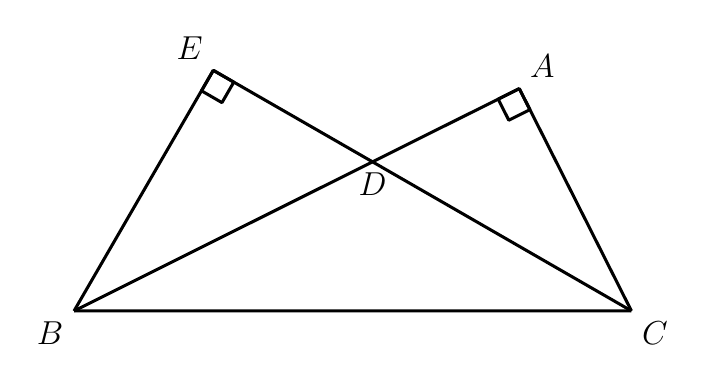
\begin{tikzpicture}[line join=round, line width=1.1pt]
  % Named points (scale s = 0.009988 cm/px, y flipped)
  \coordinate (B) at (-3.539,-1.528);
  \coordinate (C) at (3.540,-1.527);
  \coordinate (A) at (2.116,1.296);
  \coordinate (E) at (-1.770,1.528);
  \coordinate (D) at (0.252,0.366);

  % Segments (D lies on BA and EC, so they pass through D)
  \draw (B) -- (C);
  \draw (B) -- (E);
  \draw (E) -- (D) -- (C);
  \draw (B) -- (D) -- (A);
  \draw (A) -- (C);

  % Right-angle mark at A (between AB and AC), side 0.3 cm
  \draw (2.116,1.296) -- (1.848,1.162) -- (1.983,0.894) -- (2.251,1.028) -- cycle;

  % Right-angle mark at E (between EB and EC), side 0.3 cm
  \draw (-1.770,1.528) -- (-1.920,1.268) -- (-1.660,1.118) -- (-1.510,1.378) -- cycle;

  % Labels
  \node[above right] at (A) {\fontsize{11.5}{13.8}\selectfont $A$};
  \node[below left]  at (B) {\fontsize{11.5}{13.8}\selectfont $B$};
  \node[below right] at (C) {\fontsize{11.5}{13.8}\selectfont $C$};
  \node[below]       at (D) {\fontsize{11.5}{13.8}\selectfont $D$};
  \node[above left]  at (E) {\fontsize{11.5}{13.8}\selectfont $E$};
\end{tikzpicture}
\end{document}